\PassOptionsToPackage{unicode=true}{hyperref} % options for packages loaded elsewhere
\PassOptionsToPackage{hyphens}{url}
%
\documentclass[12pt,]{book}
\usepackage{lmodern}
\usepackage{amssymb,amsmath}
\usepackage{ifxetex,ifluatex}
\usepackage{fixltx2e} % provides \textsubscript
\ifnum 0\ifxetex 1\fi\ifluatex 1\fi=0 % if pdftex
  \usepackage[T1]{fontenc}
  \usepackage[utf8]{inputenc}
  \usepackage{textcomp} % provides euro and other symbols
\else % if luatex or xelatex
  \usepackage{unicode-math}
  \defaultfontfeatures{Ligatures=TeX,Scale=MatchLowercase}
\fi
% use upquote if available, for straight quotes in verbatim environments
\IfFileExists{upquote.sty}{\usepackage{upquote}}{}
% use microtype if available
\IfFileExists{microtype.sty}{%
\usepackage[]{microtype}
\UseMicrotypeSet[protrusion]{basicmath} % disable protrusion for tt fonts
}{}
\IfFileExists{parskip.sty}{%
\usepackage{parskip}
}{% else
\setlength{\parindent}{0pt}
\setlength{\parskip}{6pt plus 2pt minus 1pt}
}
\usepackage{hyperref}
\hypersetup{
            pdftitle={Geométria analítica},
            pdfauthor={Ricardo Michel MALLQUI BAÑOS},
            pdfborder={0 0 0},
            breaklinks=true}
\urlstyle{same}  % don't use monospace font for urls
\usepackage{color}
\usepackage{fancyvrb}
\newcommand{\VerbBar}{|}
\newcommand{\VERB}{\Verb[commandchars=\\\{\}]}
\DefineVerbatimEnvironment{Highlighting}{Verbatim}{commandchars=\\\{\}}
% Add ',fontsize=\small' for more characters per line
\usepackage{framed}
\definecolor{shadecolor}{RGB}{248,248,248}
\newenvironment{Shaded}{\begin{snugshade}}{\end{snugshade}}
\newcommand{\AlertTok}[1]{\textcolor[rgb]{0.94,0.16,0.16}{#1}}
\newcommand{\AnnotationTok}[1]{\textcolor[rgb]{0.56,0.35,0.01}{\textbf{\textit{#1}}}}
\newcommand{\AttributeTok}[1]{\textcolor[rgb]{0.77,0.63,0.00}{#1}}
\newcommand{\BaseNTok}[1]{\textcolor[rgb]{0.00,0.00,0.81}{#1}}
\newcommand{\BuiltInTok}[1]{#1}
\newcommand{\CharTok}[1]{\textcolor[rgb]{0.31,0.60,0.02}{#1}}
\newcommand{\CommentTok}[1]{\textcolor[rgb]{0.56,0.35,0.01}{\textit{#1}}}
\newcommand{\CommentVarTok}[1]{\textcolor[rgb]{0.56,0.35,0.01}{\textbf{\textit{#1}}}}
\newcommand{\ConstantTok}[1]{\textcolor[rgb]{0.00,0.00,0.00}{#1}}
\newcommand{\ControlFlowTok}[1]{\textcolor[rgb]{0.13,0.29,0.53}{\textbf{#1}}}
\newcommand{\DataTypeTok}[1]{\textcolor[rgb]{0.13,0.29,0.53}{#1}}
\newcommand{\DecValTok}[1]{\textcolor[rgb]{0.00,0.00,0.81}{#1}}
\newcommand{\DocumentationTok}[1]{\textcolor[rgb]{0.56,0.35,0.01}{\textbf{\textit{#1}}}}
\newcommand{\ErrorTok}[1]{\textcolor[rgb]{0.64,0.00,0.00}{\textbf{#1}}}
\newcommand{\ExtensionTok}[1]{#1}
\newcommand{\FloatTok}[1]{\textcolor[rgb]{0.00,0.00,0.81}{#1}}
\newcommand{\FunctionTok}[1]{\textcolor[rgb]{0.00,0.00,0.00}{#1}}
\newcommand{\ImportTok}[1]{#1}
\newcommand{\InformationTok}[1]{\textcolor[rgb]{0.56,0.35,0.01}{\textbf{\textit{#1}}}}
\newcommand{\KeywordTok}[1]{\textcolor[rgb]{0.13,0.29,0.53}{\textbf{#1}}}
\newcommand{\NormalTok}[1]{#1}
\newcommand{\OperatorTok}[1]{\textcolor[rgb]{0.81,0.36,0.00}{\textbf{#1}}}
\newcommand{\OtherTok}[1]{\textcolor[rgb]{0.56,0.35,0.01}{#1}}
\newcommand{\PreprocessorTok}[1]{\textcolor[rgb]{0.56,0.35,0.01}{\textit{#1}}}
\newcommand{\RegionMarkerTok}[1]{#1}
\newcommand{\SpecialCharTok}[1]{\textcolor[rgb]{0.00,0.00,0.00}{#1}}
\newcommand{\SpecialStringTok}[1]{\textcolor[rgb]{0.31,0.60,0.02}{#1}}
\newcommand{\StringTok}[1]{\textcolor[rgb]{0.31,0.60,0.02}{#1}}
\newcommand{\VariableTok}[1]{\textcolor[rgb]{0.00,0.00,0.00}{#1}}
\newcommand{\VerbatimStringTok}[1]{\textcolor[rgb]{0.31,0.60,0.02}{#1}}
\newcommand{\WarningTok}[1]{\textcolor[rgb]{0.56,0.35,0.01}{\textbf{\textit{#1}}}}
\usepackage{longtable,booktabs}
% Fix footnotes in tables (requires footnote package)
\IfFileExists{footnote.sty}{\usepackage{footnote}\makesavenoteenv{longtable}}{}
\usepackage{graphicx,grffile}
\makeatletter
\def\maxwidth{\ifdim\Gin@nat@width>\linewidth\linewidth\else\Gin@nat@width\fi}
\def\maxheight{\ifdim\Gin@nat@height>\textheight\textheight\else\Gin@nat@height\fi}
\makeatother
% Scale images if necessary, so that they will not overflow the page
% margins by default, and it is still possible to overwrite the defaults
% using explicit options in \includegraphics[width, height, ...]{}
\setkeys{Gin}{width=\maxwidth,height=\maxheight,keepaspectratio}
\setlength{\emergencystretch}{3em}  % prevent overfull lines
\providecommand{\tightlist}{%
  \setlength{\itemsep}{0pt}\setlength{\parskip}{0pt}}
\setcounter{secnumdepth}{5}
% Redefines (sub)paragraphs to behave more like sections
\ifx\paragraph\undefined\else
\let\oldparagraph\paragraph
\renewcommand{\paragraph}[1]{\oldparagraph{#1}\mbox{}}
\fi
\ifx\subparagraph\undefined\else
\let\oldsubparagraph\subparagraph
\renewcommand{\subparagraph}[1]{\oldsubparagraph{#1}\mbox{}}
\fi

% set default figure placement to htbp
\makeatletter
\def\fps@figure{htbp}
\makeatother

\usepackage{etoolbox}
\makeatletter
\providecommand{\subtitle}[1]{% add subtitle to \maketitle
  \apptocmd{\@title}{\par {\large #1 \par}}{}{}
}
\makeatother
\usepackage[spanish,es-noquoting]{babel}
% \usepackage[utf8]{inputenc}
\usepackage{amsfonts}
\usepackage{fontenc}
%\usepackage{fontspec}
\usepackage{booktabs,longtable}
%\usepackage[referable]{threeparttablex}
\usepackage{dsfont}
\usepackage[a4paper]{geometry}
\geometry{tmargin=2.5cm,bmargin=2.5cm,lmargin=3cm,rmargin=2.5cm}
%\usepackage{times}
%\renewcommand{\rmdefault}{ptm}
%\usepackage[lite,subscriptcorrection,nofontinfo,zswash]{mtpro2}
\usepackage{textcase}
\usepackage{makecell}
\usepackage{lscape}
\usepackage{multirow}
\usepackage{tabto}
%\usepackage{bigstrut}

%\DeclareFontFamily{U}{mt2ms}{\skewchar\font42}%
%\DeclareFontShape{U}{mt2ms}{m}{n}{<-7>mt2mcf<7-9>mt2mcs<9->mt2mct}{}%
%\DeclareFontShape{U}{mt2ms}{m}{it}{<-7>mt2msf<7-9>mt2mss<9->mt2mst}{}%
%\DeclareFontShape{U}{mt2ms}{b}{it}{<-7>mt2bmsf<7-9>mt2bmss<9->mt2bmst}{}%

%\usepackage{titlesec}
%\titlespacing*{\chapter}
%{0pt}{5em plus .01em minus .01em}{0em plus .01em minus .01em}
%\titlespacing*{\section}
%{0pt} {0em plus .01em minus .01em} {0em plus .01em minus .01em}
%\titlespacing*{\subsection}
%{0pt} {0em plus .01em minus .01em} {0em plus .01em minus .01em}
%\titlespacing*{\subsubsection}
%{0pt} {0em plus .01em minus .01em} {0em plus .01em minus .01em}
%\titlespacing*{\paragraph} {0pt}{1.25ex plus 1ex minus .2ex}{2em}
%\titlespacing*{\subparagraph} {\parindent}{3.25ex plus 1ex minus .2ex}{1em}
%\titleformat*{\section}{\normalsize\bfseries}
%\titleformat*{\subsection}{\normalsize\bfseries}
%\setlength{\parskip}{0.7em plus .01em minus .01em}

%%%%%%%%%%%%%%%%%%%%%%%%%%
\usepackage{xpatch}%space equation
\xapptocmd\normalsize{%
\abovedisplayskip=0.5em plus 0.01em minus 0.01em
\abovedisplayshortskip=0.5em plus 0.01em minus 0.01em
\belowdisplayskip=0.5em plus 0.01em minus 0.01em
\belowdisplayshortskip=0.5em plus 0.01em minus 0.01em
}{}{}
%%%%%%%%%%%%%%%%%%%%%
%\providecommand{\abs}[1]{\lvert#1\rvert}
%\providecommand{\norm}[1]{\lVert#1\rVert}

%\renewcommand{\thechapter}{\Roman{chapter}}

%\titleformat{\chapter}[display]
%{\normalfont\normalsize\bfseries\centering}{CAPÍTULO \thechapter}{0.0em}{\normalsize\bfseries}
%\renewcommand{\thechapter}{\Roman{chapter}}
%\renewcommand{\thesection}{\arabic{chapter}.\arabic{section}}
%\renewcommand{\thesubsection}{\arabic{chapter}.\arabic{section}.\arabic{subsection}}
%\renewcommand{\thesubsubsection}{\arabic{chapter}.\arabic{section}.\arabic{subsection}.\arabic{subsubsection}}
% https://github.com/rstudio/rmarkdown/issues/337
\let\rmarkdownfootnote\footnote%
\def\footnote{\protect\rmarkdownfootnote}

% https://github.com/rstudio/rmarkdown/pull/252
\usepackage{titling}
\setlength{\droptitle}{-2em}

\pretitle{\vspace{\droptitle}\centering\huge}
\posttitle{\par}

\preauthor{\centering\large\emph}
\postauthor{\par}

\predate{\centering\large\emph}
\postdate{\par}
\usepackage[]{natbib}
\bibliographystyle{apalike}

\title{Geométria analítica}
\author{Ricardo Michel MALLQUI BAÑOS}
\date{2020-02-16}

\usepackage{amsthm}
\newtheorem{theorem}{Teorema}[chapter]
\newtheorem{lemma}{Lema}[chapter]
\newtheorem{corollary}{Corolario}[chapter]
\newtheorem{proposition}{Proposición}[chapter]
\newtheorem{conjecture}{Conjectura}[chapter]
\theoremstyle{definition}
\newtheorem{definition}{Definición}[chapter]
\theoremstyle{definition}
\newtheorem{example}{Ejemplo}[chapter]
\theoremstyle{definition}
\newtheorem{exercise}{Ejercicio}[chapter]
\theoremstyle{remark}
\newtheorem*{remark}{Observación}
\newtheorem*{solution}{Solución}
\let\BeginKnitrBlock\begin \let\EndKnitrBlock\end
\begin{document}
\maketitle

{
\setcounter{tocdepth}{1}
\tableofcontents
}
\newcommand{\N}{\mathbb{N}}
\newcommand{\R}{\mathbb{R}}
\newcommand{\CC}{\mathbb{C}}
\newcommand{\I}{\mathbb{I}}
\newcommand{\f}{\mathbb{f}}
\newcommand{\X}{\mathbb{X}}
\newcommand{\D}{\mathbb{D}}
\newcommand{\Z}{\mathbb{Z}}
\newcommand{\Q}{\mathbb{Q}}
\newcommand{\norm}[1]{\left\Vert#1\right\Vert}
\newcommand{\abs}[1]{\left\vert#1\right\vert}
\newcommand{\set}[1]{\left\{#1\right\}}
\newcommand{\seq}[1]{\left<#1\right>}
\newcommand{\co}[1]{\left[#1\right]}
\newcommand{\cc}[1]{\left(#1\right)}
\newcommand{\J}{\mathcal{J}}
\newcommand{\K}{\mathcal{K}}
\newcommand{\M}{\mathcal{M}}
\newcommand{\F}{\mathcal{F}}

\hypertarget{prerequisitos}{%
\chapter{Prerequisitos}\label{prerequisitos}}

See Theorem \ref{thm:boring} \[\sum_1^2\]

\BeginKnitrBlock{theorem}
\protect\hypertarget{thm:boring}{}{\label{thm:boring} }Here is my theorem.
\EndKnitrBlock{theorem}

\BeginKnitrBlock{definition}[ww]
\protect\hypertarget{def:unnamed-chunk-1}{}{\label{def:unnamed-chunk-1} \iffalse (ww) \fi{} }
\EndKnitrBlock{definition}

See Figure \ref{fig:cars-plot} \ref{fig:pressure}

\begin{Shaded}
\begin{Highlighting}[]
\KeywordTok{plot}\NormalTok{(cars)  }\CommentTok{# a scatterplot}
\end{Highlighting}
\end{Shaded}

\begin{figure}
\centering
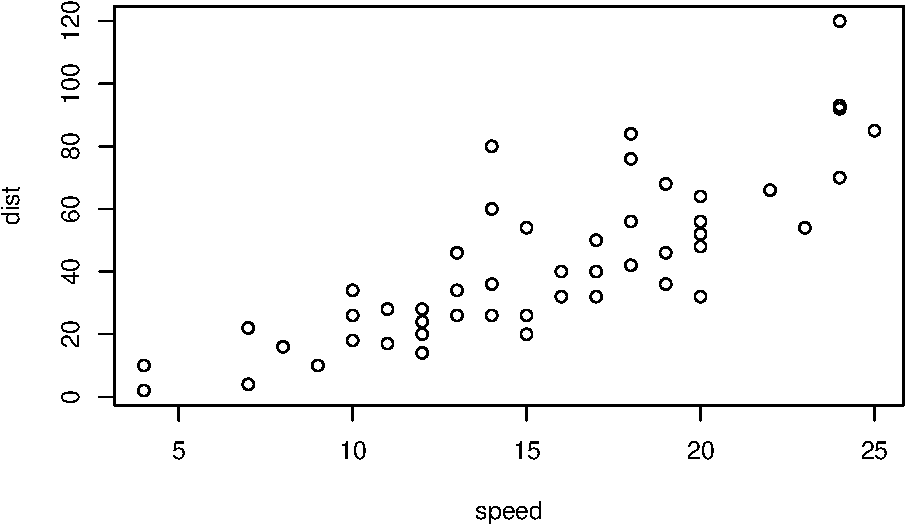
\includegraphics{uu_files/figure-latex/cars-plot-1.pdf}
\caption{\label{fig:cars-plot}A plot caption}
\end{figure}

\BeginKnitrBlock{theorem}[Pythagorean theorem]
\protect\hypertarget{thm:pyth}{}{\label{thm:pyth} \iffalse (Pythagorean theorem) \fi{} }For a right triangle, if \(c\) denotes the length of the hypotenuse
and \(a\) and \(b\) denote the lengths of the other two sides, we have

\[a^2 + b^2 = c^2\]
\EndKnitrBlock{theorem}

See Table \ref{tab:mtcars}

\begin{figure}

{\centering 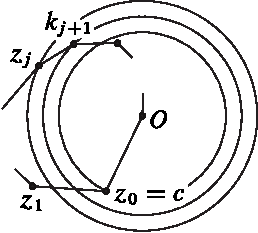
\includegraphics[width=1\linewidth]{inverse} 

}

\caption{A caption}\label{fig:pressure}
\end{figure}

\begin{Shaded}
\begin{Highlighting}[]
\NormalTok{knitr}\OperatorTok{::}\KeywordTok{kable}\NormalTok{(mtcars[}\DecValTok{1}\OperatorTok{:}\DecValTok{5}\NormalTok{, }\DecValTok{1}\OperatorTok{:}\DecValTok{5}\NormalTok{], }\DataTypeTok{caption =} \StringTok{"A caption"}\NormalTok{, }\DataTypeTok{booktabs=}\OtherTok{TRUE}\NormalTok{)}
\end{Highlighting}
\end{Shaded}

\begin{table}

\caption{\label{tab:mtcars}A caption}
\centering
\begin{tabular}[t]{lrrrrr}
\toprule
  & mpg & cyl & disp & hp & drat\\
\midrule
Mazda RX4 & 21.0 & 6 & 160 & 110 & 3.90\\
Mazda RX4 Wag & 21.0 & 6 & 160 & 110 & 3.90\\
Datsun 710 & 22.8 & 4 & 108 & 93 & 3.85\\
Hornet 4 Drive & 21.4 & 6 & 258 & 110 & 3.08\\
Hornet Sportabout & 18.7 & 8 & 360 & 175 & 3.15\\
\bottomrule
\end{tabular}
\end{table}

\begin{equation} 
  f\left(k\right) = \binom{n}{k} p^k\left(1-p\right)^{n-k}
  \label{eq:binom}
\end{equation}

Este es un \emph{ejemplo} book written in \textbf{Markdown} \eqref{eq:binom}. You can use anything that Pandoc's Markdown supports, e.g., a math equation \(a^2 + b^2 = c^2\).

The \textbf{bookdown} package can be installed from CRAN or Github:

\begin{Shaded}
\begin{Highlighting}[]
\KeywordTok{install.packages}\NormalTok{(}\StringTok{"bookdown"}\NormalTok{)}
\CommentTok{# or the development version}
\CommentTok{# devtools::install_github("rstudio/bookdown")}
\end{Highlighting}
\end{Shaded}

Remember each Rmd file contains one and only one chapter, and a chapter is defined by the first-level heading \texttt{\#}.

To compile this example to PDF, you need XeLaTeX. You are recommended to install TinyTeX (which includes XeLaTeX): \url{https://yihui.org/tinytex/}.

\hypertarget{intro}{%
\chapter{Introduction}\label{intro}}

\BeginKnitrBlock{theorem}[russ]
\protect\hypertarget{thm:www}{}{\label{thm:www} \iffalse (russ) \fi{} }Dada el espacio \(R\) y \(r\in R\) se tiene que \(\mathcal{R}(r)=\lim_{t\to\infty}g(y)_r\)
\EndKnitrBlock{theorem}

\BeginKnitrBlock{proof}
\iffalse{} {Demostracion. } \fi{}En efecto haciendo el intercambio de variables se tiene que \(\sum_{i=1}^{\infty}r_i\)
\[\vec{r}=\left\vert\frac{\vec{\int_1^2r}}{\left|r_1^2\right|}\right\vert\left\Vert\int_1^2e\right\Vert\]
por lo tanto se cumple.
\EndKnitrBlock{proof}

You can label chapter and section titles using \texttt{\{\#label\}} after them, e.g., we can reference Chapter \ref{intro}. If you do not manually label them, there will be automatic labels anyway, e.g., Chapter \ref{methods}.

Figures and tables with captions will be placed in \texttt{figure} and \texttt{table} environments, respectively.

\begin{Shaded}
\begin{Highlighting}[]
\KeywordTok{par}\NormalTok{(}\DataTypeTok{mar =} \KeywordTok{c}\NormalTok{(}\DecValTok{4}\NormalTok{, }\DecValTok{4}\NormalTok{, }\FloatTok{.1}\NormalTok{, }\FloatTok{.1}\NormalTok{))}
\KeywordTok{plot}\NormalTok{(pressure, }\DataTypeTok{type =} \StringTok{'b'}\NormalTok{, }\DataTypeTok{pch =} \DecValTok{19}\NormalTok{)}
\end{Highlighting}
\end{Shaded}

\begin{figure}

{\centering 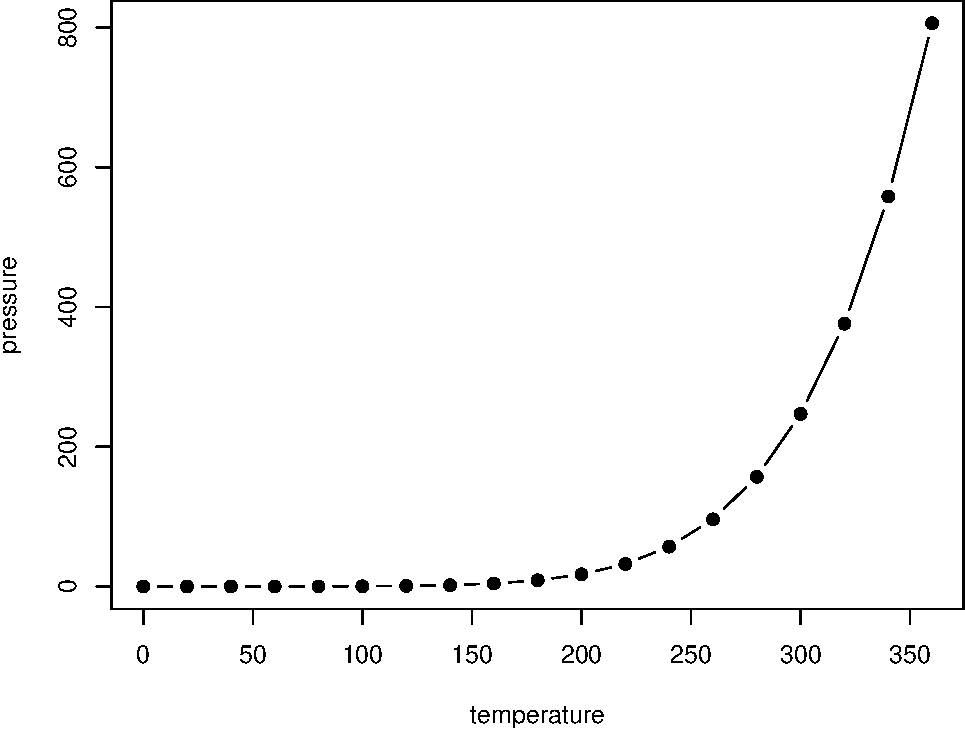
\includegraphics[width=0.8\linewidth]{uu_files/figure-latex/nice-fig-1} 

}

\caption{Here is a nice figure!}\label{fig:nice-fig}
\end{figure}

Reference a figure by its code chunk label with the \texttt{fig:} prefix, e.g., see Figure \ref{fig:nice-fig}. Similarly, you can reference tables generated from \texttt{knitr::kable()}, e.g., see Table \ref{tab:nice-tab}.

\begin{Shaded}
\begin{Highlighting}[]
\NormalTok{knitr}\OperatorTok{::}\KeywordTok{kable}\NormalTok{(}
  \KeywordTok{head}\NormalTok{(iris, }\DecValTok{20}\NormalTok{), }\DataTypeTok{caption =} \StringTok{'Here is a nice table!'}\NormalTok{,}
  \DataTypeTok{booktabs =} \OtherTok{TRUE}
\NormalTok{)}
\end{Highlighting}
\end{Shaded}

\begin{table}

\caption{\label{tab:nice-tab}Here is a nice table!}
\centering
\begin{tabular}[t]{rrrrl}
\toprule
Sepal.Length & Sepal.Width & Petal.Length & Petal.Width & Species\\
\midrule
5.1 & 3.5 & 1.4 & 0.2 & setosa\\
4.9 & 3.0 & 1.4 & 0.2 & setosa\\
4.7 & 3.2 & 1.3 & 0.2 & setosa\\
4.6 & 3.1 & 1.5 & 0.2 & setosa\\
5.0 & 3.6 & 1.4 & 0.2 & setosa\\
\addlinespace
5.4 & 3.9 & 1.7 & 0.4 & setosa\\
4.6 & 3.4 & 1.4 & 0.3 & setosa\\
5.0 & 3.4 & 1.5 & 0.2 & setosa\\
4.4 & 2.9 & 1.4 & 0.2 & setosa\\
4.9 & 3.1 & 1.5 & 0.1 & setosa\\
\addlinespace
5.4 & 3.7 & 1.5 & 0.2 & setosa\\
4.8 & 3.4 & 1.6 & 0.2 & setosa\\
4.8 & 3.0 & 1.4 & 0.1 & setosa\\
4.3 & 3.0 & 1.1 & 0.1 & setosa\\
5.8 & 4.0 & 1.2 & 0.2 & setosa\\
\addlinespace
5.7 & 4.4 & 1.5 & 0.4 & setosa\\
5.4 & 3.9 & 1.3 & 0.4 & setosa\\
5.1 & 3.5 & 1.4 & 0.3 & setosa\\
5.7 & 3.8 & 1.7 & 0.3 & setosa\\
5.1 & 3.8 & 1.5 & 0.3 & setosa\\
\bottomrule
\end{tabular}
\end{table}

You can write citations, too. For example, we are using the \textbf{bookdown} package \citep{R-bookdown} in this sample book, which was built on top of R Markdown and \textbf{knitr} \citep{xie2015}.

\hypertarget{literature}{%
\chapter{Literature}\label{literature}}

Here is a review of existing methods.

\hypertarget{methods}{%
\chapter{Methods}\label{methods}}

We describe our methods in this chapter.

\hypertarget{applications}{%
\chapter{Applications}\label{applications}}

Some \emph{significant} applications are demonstrated in this chapter.

\hypertarget{example-one}{%
\section{Example one}\label{example-one}}

\hypertarget{example-two}{%
\section{Example two}\label{example-two}}

\hypertarget{final-words}{%
\chapter{Final Words}\label{final-words}}

We have finished a nice book.

\bibliography{book.bib,packages.bib}

\end{document}
